\documentclass[a4paper, 12pt]{article} % тип документа
\usepackage[T2A]{fontenc} % Поддержка русских букв
\usepackage[utf8]{inputenc} % кодировка 
\usepackage[english,russian]{babel} % языковой пакет
\usepackage{amsmath,amsfonts, amssymb} % шрифты
\usepackage[colorlinks,urlcolor=blue]{hyperref} % для гиперссылок
\usepackage{anysize} % для отступов	
\usepackage{setspace} % интервал
\usepackage{dsfont} % индикатор
\usepackage{color}
\usepackage{textcomp}
\usepackage{graphicx}
\onehalfspacing % уточняет интервал
\usepackage{indentfirst} % чтобы первый абзац в разделе тоже был с отступом
\marginsize{2.5cm}{2cm}{1cm}{1cm} % поля
\usepackage{amsthm} % работа с теоремами
\newtheorem{statement}{Утверждение}
\usepackage[colorlinks=true,urlcolor=black]{hyperref}
\hypersetup{linkcolor = black, hidelinks}
\usepackage{afterpage}
\usepackage{listings}
\usepackage{caption} % multiline caption



\makeatletter
\renewcommand{\@biblabel}[1]{#1.} % Заменяем библиографию с квадратных скобок на точку:
\makeatother

% блок-схема
\usepackage{tikz}
\usetikzlibrary{shapes, arrows}
\tikzstyle{decision} =
        [
                diamond,
                draw,
                text width = 6em,
                text badly centered,
                node distance = 3cm,
                inner sep = 0pt
        ]
\tikzstyle{block} =
        [
                rectangle,
                draw,
                text width = 10em,
                text centered,
                rounded corners,
                minimum height = 3em
        ]
\tikzstyle{line} =
        [
                draw,
                -latex'
        ]
\tikzstyle{cloud} =
        [
                draw,
                ellipse,
                node distance = 3cm,
                minimum height = 2em,
                text width = 12em,
        ]

%\title{Построение рекомендательной системы, основанной на итерационном улучшении качества классификации}
%\author{Ведерников А.В.}

\begin{document}

%\usepackage{graphicx}

%%%%%%%%%%%%%%%%%%%%%%%%%%%
%\usepackage{srcltx}
%%%%%%%%%%%%%%%%%%%%%%%%%%%%%%

\begin{titlepage}

\large \thispagestyle{empty} \phantom{.}\vspace{2mm} \large
\thispagestyle{empty}

\begin{center}
%МИНИСТЕРСТВО НАУКИ И ОБРАЗОВАНИЯ\\
%РОССИЙСКОЙ ФЕДЕРАЦИИ\\
%\bigskip
МОСКОВСКИЙ ГОСУДАРСТВЕННЫЙ УНИВЕРСИТЕТ\\
ИМ. М.В.ЛОМОНОСОВА\\
\noindent\

\vspace{0.3cm}

\vspace{-0.8cm}
МЕХАНИКО--МАТЕМАТИЧЕСКИЙ ФАКУЛЬТЕТ\\

\vspace{0.8cm}



\end{center}
%\vfill
\newline
\begin{center}
Кафедра математической теории интеллектуальных систем
\end{center}

%\begin{center}
%{\Large \bf Чечкин Григорий Александрович}
%\end{center}
%\bigskip
%\bigskip

\begin{figure}[htbp] %htbp

\begin{center}


\includegraphics[width=6cm]{mmlogo1}

\end{center}

\end{figure}


\begin{center}
{\LARGE \bf ПОСТРОЕНИЕ РЕКОМЕНДАТЕЛЬНОЙ СИСТЕМЫ, ОСНОВАННОЙ НА ИТЕРАЦИОННОМ УЛУЧШЕНИИ ТОЧНОСТИ КЛАССИФИКАЦИИ\\
%\medskip
}\\
%\bigskip
%\medskip
%01.01.02 — дифференциальные уравнения
\end{center}
\vfill


\bigskip
\begin{flushright}
Дипломная работа студента группы 511\\
 Ведерникова Артема Викторовича\\
Научный руководитель:\\ к.т.н., к.ф.-м.н., доцент \\Рыжов А.П.\\
Рецензент: \\к.ф.-м.н., м.н.с. \\
Шуткин Ю.С. 
\end{flushright}
\vfill \vfill \centerline{Москва 2014} \break
\end{titlepage}

\tableofcontents

\newpage
\section{Аннотация}
Быстрое развитие Интернет-технологий и увеличение объемов информации в Сети в последнее десятилетие привело к развитию такого вида веб-сервисов, как рекомендательные системы. Они облегчают процесс поиска, предлагая информацию, которая может быть интересна пользователю, исходя из истории его взаимодействий с системой. Одной из главных проблем рекомендательных систем является низкое качество предложенных рекомендаций при высокой разреженности входных данных. Для решения данной проблемы в работе рассмотрен рекомендательный алгоритм, основанный на методе коллаборативной фильтрации. Улучшение качества рекомендаций при сильно разреженных входных данных достигается за счет пошаговой оценки части неизвестных рейтингов и кластеризации множества пользователей. Проведено тестирование алгоритма и сравнение его с другими широко используемыми рекомендательными методами.

\newpage
\section{Введение}
В настоящее время количество доступной информации в сети Интернет стремительно растет, вследствие чего задача предоставления пользователю данных, соответстветствующих его запросам и предпочтениям, становится одной из самых важных при создании веб-сервиса. Именно поэтому большинство крупнейших сайтов Сети представляют из себя именно поисковые системы, например, Google, Yahoo, Yandex. Другим широким классом сервисов, облегчающих поиск информации, являются рекомендательные системы. Они представляют из себя программы, которые, используя информацию о пользователе и его предпочтениях, помогают в выборе подходящих объектов из некоторой библиотеки\cite{cfdef}.  Это могут быть фильмы (Netflix), товары (Amazon), музыкальные исполнители (Last.fm). В процессе вычисления рекомендаций эти системы используют оценки, проставленные пользователями, а также информацию о пользователях и рекомендуемых объектах. 


\par
Существует несколько базовых подходов к построение рекомендательных систем: алгоритмы, основанные на анализе содержания (Content-based), алгоритмы, анализирующие схожесть предпочтений пользователей --- коллаборативная фильтрация (Collaborative filtering) и гибридные алгоритмы. 
\par
Системы, основанные на \textit{анализе содержания}, при прогнозировании оценок сопоставляют информацию о рекомендуемых объектах (жанр, автор, год выпуска и т.д.) с информацией об уже оцененных пользователем объектах. Пользователю предлагаются объекты, схожие с теми, которые он отметил как понравившиеся. Для поиска часто используются ключевые слова, хеш-теги. 
\par
Основная идея алгоритма \textit{коллаборативной фильтрации} заключается в предложении новых объектов для конкретного пользователя на основе оценок, проставленных <<похожими>> пользователями --- коллаборативная фильтрация, основанная на сходстве пользователей, либо на основе оценок, поставленных объектам, <<похожим>> на те, что положительно оценил пользователь --- коллаборативная фильтрация, основанная на сходстве объектов. Мера близости пользователей и/или объектов зависит от конкретной реализации. 
\par
Алгоритмы коллаборативной фильтрации могут основываться либо на анализе имеющих оценок (memory-based), либо на построении и анализе некоторой модели данных (model based). Часто при построении рекомендательных систем эти подходы объединяются. Рассмотрим виды коллаборативной фильтрации подробнее.
\par
Первая группа алгоритмов на начальном этапе работы оценивает степень схожести между пользователями и/или рекомендуемыми объектами. Далее происходит отбор наиболее похожих пользователей (объектов) --- ближайших соседей, недостающие рейтинги оцениваются в соответствии с их оценками. 
\par
Методы второй группы на первом этапе строят статистическую модель оценок пользователей, которая обучается на тренировочном раборе данных, после чего используется для оценки. Здесь широко используются различные алгоритмы кластеризации, байесовские сети, а также методы уменьшения размерности данных и разложения матриц (SVD). Алгоритмы, основанные на построении  модели, показывают высокие результаты при работе с сильно разреженными данными. Недостатки модели связаны с необходимостью соблюдения компромисса между точностью оценок и размером модели.

\par
Гибридные рекомендательные системы сочетают в себе несколько различных подходов к оценке неизвестных рейтингов и подразделяются на параллельные, последовательные и монолитные. В параллельных системах оценки вычисляются как линейные комбинации результатов, полученных при независимой работе нескольких рекомендательных алгоритмов. В последовательных системах результат работы одного алгоритма используется в качестве входных данных для другого. Монолитные рекомендательные  системы используют несколько подходов в рамках единого алгоритма, не позволяя изолированно рассматривать результаты работы конкретного метода.

\par 
Одним из главных недостатков как алгоритмов, основанных на анализе содержания, так и коллаборативной фильтрации является проблема выдачи релевантных рекомендаций для новых пользователей и для новых объектов. В литературе данный недостаток называют <<проблемой холодного старта>>\cite{coldstart}. Существует множество способов ее решения, большинство из которых сводится к добавлению в систему дополнительной информации о пользователях и объектах. Например, система, разработанная для рекомендации научной литературы, может использовать информацию о совместных работах авторов\cite{socnetclust}.

\par
Еще одной проблемой большинства существующих рекомендательных алгоритмов является низкое качество рекомендаций при работе с данными высокой разреженности. Наиболее часто используемыми методами устронения этого недостатка является добавление к данным некоторого количества стандартных рейтингов\cite{empiricalanalysis}. Тестирование показывает, что подобный подход заметно улучшает качество рекомендаций, однако его результаты сильно зависят от выбора дополнительных параметров алгоритма.  

\par
В данной работе построен \textit{новый рекомендательный алгоритм}, основной задачей которого является повышение качества рекомендаций при высокой разреженности входных данных. Метод основан на применении коллаборативной фильтрации. На каждой итерации множества схожих пользователей определяются с использованием нечеткой кластеризации, далее происходит оценка неизвестных рейтингов. Проведено тестирование и сравнение метода с другими широко используемыми рекомендательными алгоритмам, дана оценка полученных результатов.


\section{Обзор литературы}
\par 
Необходимо обратить внимание, что большая часть методов, используемых при построении рекомендательных систем носит \textit{эмпирический }характер и имеет большое число дополнительных параметров, значения которых подбираются отдельно для каждого конкретного набора данных на основе проведенных испытаний. На примере следующих статей, продемонстрированы возможные подходы к построению рекомендаций.
\subsection{Методы, использующие кластеризацию пользователей}
\par
В работе <<A new collaborative recommendation approach based on users clustering using artificial bee colony algorithm>>$\cite{bees}$ был представлен алгоритм коллаборативной фильтрации, в основе которого лежит кластеризация пользователей исходя из проставленных ими рейтингов методом k-средних с использованием алгоритма искуственной пчелиной колонии (Artificial bee colony algorithm) для определения начальных центров кластеров. В качестве меры близости пользователей внутри кластера была использована модифицированная косинусная метрика, в которую добавлен вес рекомендуемого объекта. На прогнозируемую оценку для пользователя $u \in U$  влияли только оценки пользователей одного с ним класса. Тестирование метода проводилось на наборе данных MovieLens, состоящем из 100000 оценок 943 пользователей, проставленных 1682 фильмам. Разреженность данных составляла 6,3\%. Алгоритм сравнивался с другими методами на основе коллаборативной фильтрации и показал самый высокий показатель качества рекомендаций\footnote{Методы оценки рекомендательных систем рссмотрены подробно в разделе <<Тестирование>>}.

\par 
Кольчугин и Макарь в статье <<Метод коллаборативной фильтрации для масштабируемых рекомендательных систем>>$\cite{hash}$ при построении алгоритма коллаборативной фильтрации для кластеризации пользователей используют разработанный ими алгоритм LSH-CLC, основанный на методе локально-чувствительного хеширования LSH. Этот метод используется для нахождения ближайших соседей. На основе найденных схожих пользователей впоследствии формируются кластеры. Прогнозируемые оценки для пользователя $u \in U$ рассчитываются исходя из его сходства с центроидами кластеров. В качестве меры близости между пользователями используется корреляция Пирсона. Благодаря использованию хеширования удалось достичь линейной зависимости сложности кластеризации пользователей от их общего числа \textit{n}, таким образом сложность рекомендательного алгоритма также зависит от \textit{n} линейно. Тестирование производилось на наборе данных MovieLens, содержащем 100000 оценок и имеющих разреженность 6,3\%. В тестах данный метод показал качество, близкое к SVD-алгоритму. При оценке времени работы использовались наборы данных, содержащие от 1000 до 6000 пользователей. При использовании информации о 1000 пользователях время работы алгоритма составило 5 секунд, при 4500 порядка 30 секунд, при 6000 --- около 60 секунд. Полученные результаты подтверждают линейную зависимость времени работы алгоритма от количества пользователей.  

\par В работе <<A Clustering Approach for Collaborative Filtering Recommendation Using Social Network Analysis>>$\cite{socnetclust}$ Pham, Cao, Klamma, Jarke разрабатывают рекомендательную систему, работающую по основанному на сходстве пользователей методу коллаборативной фильтрации. Задача этой системы --- рекомендация научных статей, журналов и конференций, основными пользователями являются молодые ученые и аспиранты. Отличительной особенностью является использовние информации о совместных публикациях. На основе этих данных авторы строят социальную сеть, отражающую пользовательские взаимодействия. Далее эта сеть используются для кластеризации пользователей, после чего для каждого пользователя неизвестные рейтинги оцениваются в соответствии с оценками, проставленными пользователями того же кластера. При тестировании авторы использовали данные сайта Epinion\footnote{Epinion. URL: http://www10.epinions.com}, социальная сеть пользователей строилась на основе проставленных пользователями очков <<доверия>> друг к другу. Тестовые данные содержали 49290 пользователей, 139738 объектов, 664824 пользовательских оценки и 487182 очка доверия. Разреженность матрицы рейтингов составила 0.1\%. Разработанный алгоритм сравнивался с двумя стандартными рекомендательными методами на основе коллаборативной фильтрации и показал самую высокую точность рекомендаций --- MAE = 0,84 против 0,87 и 0,93).  

\subsection{Итерационные методы}
\par
Zhang, Cuff, Kulkarni в работе <<Iterative collaborative filtering for recommender systems with sparse data>>$\cite{itercf}$ описывают алгоритм коллаборативной фильтрации, основной задачей которого является повышение качества рекомендаций при работе с данными высокой разреженности. Для этого авторы при оценке неизвестного рейтинга объекта $i \in I$ для пользователя $u \in U$ предлагают воспользоваться итерационным алгоритмом, на каждом шаге которого происходит оценка рейтингов на основе попарных расстояний между пользователями, оценки полученные на i-м шаге используются для подсчета расстояний на i+1-м. Алгоритм завершается, когда разница между значениями оценок на соседних шагах станет меньше заданного значения $\varepsilon$. При тестировании алгоритма было использовано значение $\varepsilon=0,01$. Оно было получено на основе результатов предварительной настройки и проверки алгоритма. Тестирование производилось на наборе данных MovieLens, состоящем из 100000 рейтингов, проставленных 943 пользователями 1682 фильмам. Оригинальный набор данных был дополнительно обработан с целью понизить показатель разреженности до 5\% и 1\% (Начальное значение 6.3\%). Результаты показали, что алгоритм сходится очень быстро и успешно завершается после 2-4 итераций. Помимо высокого качества работы при высокой разреженности матрицы рейтингов (1\%) , алгоритм продемонстрировал хорошие результаты и при умеренной разреженности (6,3\%), уступив только модифицированному с использованием коллаборативной фильтрации SVD-алгоритму\cite{cfbasedsvd}.

\par
Статья <<Iterative smoothing technique for improving stability of recommender system>>$\cite{smoothing}$ посвящена алгоритму итерационного сглаживания для увеличения стабильности рекомендательных систем. Этот метод используется совместно с любым другим рекомендательным алгоритмом. Использование такого подхода позволяет повысить качество и стабильность рекомендаций\footnote{}. Метод состоит в следующем: на первом шаге неизвестные рейтинги оцениваются с использованием базового алгоритма Т, далее в течение K итераций полученные на предыдущем шаге оценки добавлялись ко входным данным, после чего происходила переоценка рейтингов с использованием расширенных входных данных. Оптимальное значение K вычисляется отдельно для каждого набора тестовых данных методов на основе полученных результатов. На стадии тестирования авторы сравнивали результаты работы различных рекомендательных алгоритмов в паре с описанным методом и без него. Среди рассмотренных методов присутстствовали SVD и основанная как на пользователях, так и на объектах коллаборативная фильтрация. В качестве тестовых данных, как и в рассмотренных выше работах, использовались данные MovieLens, содержащие 100000 и 400627 рейтингов с разреженностью 6,3\% и 4,45\% соответственно, а также данные сайта Netflix, содержащие 105256 рейтингов, разреженность составила 1,17\%. При использовании итеративного сглаживания на всех наборах данных у всех базовых алгоритмов было отмечено улучшение показателей стабильности (приблизительно на 50\% у методов коллаборативной фильтрации, на 14\% у SVD) и качества рекомендаций (в среднем на 1,4\%). 

\subsection{Заключение к обзору литературы}
Были рассмотрены работы, посвященные двум широко используемым подходам к построению рекомендательных систем: кластеризация пользователей и итерационный процесс подсчета оценок неизвестных рейтингов. Особенностью алгоритма, представленного в данной работе, является сочетание обеих описанных методик: на каждой итерации оценка рейтингов происходит в зависимости проведенной кластеризации объектов. 


\section{Методология и формулировка задачи}
\subsection{Формулировка задачи}
Имеется конечный набор объектов $I=\{i_{1}, i_{2}, \dots, i_{m}\}$ и конечный набор пользователей $U=\{u_{1}, u_{2}, \dots, u_{n}\}$.
Положим $r_{ui}$ --- рейтинг, который пользователь $u\in U$ поставил объекту $i\in I$. Как правило, рейтингами являются натуральные числа. Если пользователь $u \in U$ не оценил объект $i \in I$, то обозначим $r_{ui} = \varnothing$. Тогда n x m матрицу  $R = (r_ui) $ будем называть мартицей рейтингов. Задачей рекомендательной системы является оценка неизвестных рейтингов $r_{ui}$. Пользователю рекомендуются объекты, чьи неизвестные рейтинги по результатам работы алгоритма получили самую высокую оценку.


\subsection{Функция похожести}
Важным шагом при построении рекомендательной системы является задание функции похожести между пользователями и/или объектами. Ниже приведены наиболее часто используемые функции похожести пользователей.
\begin{itemize}

\item{Корреляция Пирсона\cite{grouplens}}
%TODO: тут вставить почему она крутая(как просил Рыжов))
\[
s_{uv} = \frac{\sum_{i \in I_{uv}} (r_{ui} - \bar{r}_{u})(r_{vi} - \bar{r}_{v})}{\sqrt{\sum_{i \in I_{uv}}  (r_{ui} - \bar{r}_{u})^2} \sqrt{\sum_{i \in I_{uv}}  (r_{vi} - \bar{r}_{v})^2}},\qquad s_{uv} \in [-1, 1]
\]

$I_{uv} = \{i \in I: r_{ui} \neq  \varnothing, r_{vi} \neq \varnothing\}$ 
\\
$\bar{r}_{u}$ --- средний рейтинг, проставленный пользователем $u \in U$ 
\\ 
Большее значение коэффициента корреляции Пирсона соответствует парам объектов с большей похожестью. Проблемы могут возникать при оценке пользователей, поставивших всем объектам одинаковый рейтинг. В таком случае предлагается вычислить ковариацию двух пользователей\\ $cov(u, v) = \sum_{i \in I_{uv}} (r_{ui} - \bar{r}_{ui})(r_{vi} - \bar{r}_{vi})$ и положить $s_{uv}=sign(cos(u,v)) * 0,5$. К недостаткам корреляции Пирсона можно отнести тот факт, что на значение этой функции похожести не оказывает влияние количество одинаково оцененных объектов у двух пользователей.


\item{Косинусное расстояние}

\[
s_{uv} = \frac{\sum_{i \in I_{uv}} r_{ui}r_{vi}} {\sqrt{\sum_{i \in I_{uv}} r_{ui}^2} \sqrt{\sum_{i \in I_{uv}} r_{vi}^2}},\qquad s_{uv} \in [-1, 1] 
\]

При использовании косинусного расстояния множество оценок, проставленных пользователями, рассматривается как вектор в $|I|$ - мерном пространстве, а мерой похожести является угол между этими векторами. Большее значение косинусного расстояния соответствует парам пользователей с большей похожестью. 
\end{itemize}

Мера похожести для объектов $\hat{s}_{ij}, \{i, j\} \subset I$ может быть подсчитана аналогично. Например, для коэффициента корреляции Пирсона формула имеет вид

\[
	\hat{s}_{ij} = \frac{\sum_{u \in U_{ij}} (r_{ui} - \bar{r}_{i})(r_{uj} - \bar{r}_{j})}{\sqrt{\sum_{u \in U_{ij}}  (r_{ui} - \bar{r}_{i})^2} \sqrt{\sum_{u \in U_{ij}}  (r_{uj} - \bar{r}_{j})^2}},\qquad \hat{s}_{uv} \in [-1, 1]
\]
\noindent
$U_{ij} = \{u \in U: r_{ui} \neq  \varnothing, r_{uj} \neq \varnothing\}$ 
\\
$\bar{r}_{i}$ --- средний рейтинг, поставленный объекту $i \in I$ 
\\ 


\subsection{Выбор ближайших соседей}
После подсчета меры близости между пользователями, алгоритмы коллаборативной фильтрации выбирают  для данного пользователя наиболее похожих на него. В работе (Zhang, Pu)\cite{neighbourhoodselection} выделяются следующие основные стратегии:
\begin{itemize}

\item Выбор K наиболее похожих пользователей

\item Выбор K наиболее похожих пользователей, оценивших выбранный объект

\item Выбор K наиболее похожих пользователей, оценивших выбранный объект и имеющих с данным пользователем не менее $p$ одинаково оцененных объектов

\item Комбинации стратегий 1, 2 и 3

\end{itemize}

Выбор метода поиска ближайших соседей зависит от выбора меры схожести, а так же от области применения рекомендательной системы. Наиболее предпочтительным является использование комбинаций стратегий.


\subsection{Оценка неизвестных рейтингов}

В алгоритмах коллаборативной фильтрации, основанных на схожести пользователей, после того, как будут найдены <<ближайшие соседи>>, неизвестные рейтинги пользователя могут оцениваться несколькими методами. 
\begin{itemize}
\item Взвешенная сумма (Weighted sum)
\[
	\hat{r}_{ui} = \bar{r}_{u} + \frac{\sum_{v \in \hat{U}_{u}} s_{uv}(r_{vi} - \bar{r}_v)}{\sum_{v \in \hat{U}_{u}} |s_{uv}|}
\]

\item Простое взвешенно среднее (Simple weighted average)
\[
	\hat{r}_{ui} = \frac{\sum_{v \in \hat{U}_{u}} r_{vi} s_{uv}}{\sum_{v \in \hat{U}_{u}}|s_{uv}|}
\]
\end{itemize}
$\hat{r}_{ui}$ --- оценка неизвестного рейтинга $r_{ui}$
\\
$s_{uv}$ --- коэффициент схожести пользователей $u$ и $v$
\\
$\hat{U}_{u}$ --- подмножество пользователей, оценивших объект $i$
\\
$\bar{r}_v$ --- среднее значение рейтинга, проставленного пользователем $v$
\par В алгоритмах коллаборативной фильтрации, основанных на схожести объектов, применяются аналогичные формулы, в которых суммирование происходит по подмножеству $\hat{ I}_{i}$ всех объектов, которые оценил пользователь $u$, а мера близости между пользователями $s_{uv}$ заменяется на меру близости между объектами $\hat{s}_{ij}, \{i, j\} \subset I$ 


\subsection{Применение кластеризации в методах коллаборативной фильтрации}
Применение кластеризации помогает заметно улучшить качество и скорость работы рекомендательной системы\cite{clustersearch}. Кластеризации могут подвергаться как пользователи\footnote{См. раздел <<Обзор литературы>>}, так и предлагаемые объекты\cite{clusteritemcf}. Одним из главных недостатков использования классических алгоритмов кластеризации в рекомендательных системах является то, что в итоге каждому объекту или пользователю приписывается только один кластер, в реальной жизни пользователи и объекты обычно принадлежат нескольким кластерам. Для решения этой проблемы для каждого объекта или пользователя расматривается множество кластеров, расстояние до центра которых меньше заданного значения. В работе предлагается использовать алгоритм нечеткой кластеризации.

\subsection{Нечеткая кластеризация}
Имеется $X=\{x_{1},\dots,x_{n}\}$ --- множество объектов,, задана функция расстояния между ними $d(x, y): X\times X  \to \mathbb{R}$ В классической задаче кластеризации требуется разбить $X$ на непересекающиеся подмножества $\{c_{1},\dots,c_{m}\} = C$,  называемые кластерами, так, чтобы каждый кластер состоял из объектов, близких по метрике $dist$, а объекты разных классов существенно отличались. При этом каждому объекту $x_{i} \in X$ приписывается единственный кластер $c_{i} \in C$, $X = \bigsqcup_{i} c_{i}$.
\par
 Особенностью нечеткой кластеризации является то, что объекту $x \in X$ приписывается не единственный кластер, а вещественный вектор $\lambda(x)=(\lambda_{1}(x),\dots,\lambda_{m}(x))$, элементами которого являются степени принадлежности $x$ кластерам из $C$. , при этом выполняются следующие условия:
 \begin{itemize}
 \item $\forall x \in X: \forall c: 1\leq c \leq m:  \lambda_{m}(x) \in [0,1]$
 \item $\forall x \in X: \sum_{j=1,\dots,c} \lambda_{j}(x) = 1$
 \item $\forall i : 0 < \sum_{j=1}^{n} \lambda_{i}(x_{j}) < |X|  $
 \end{itemize} 
 \par
 В работе используется метод нечеткой классификации FANNY (Kaufman, Rousseeuw)$\cite{fanny}$. Этот алгоритм основывается на минимизации функции 
\[
	V=\sum_{v=1..k} \frac{\sum_{i,j} \lambda_{v}^r(i) \lambda_{v}^r(j) dist(i,j)}{2 \sum_{j} \lambda_{v}^r(j)}
\]
где k --- число кластеров, задается как параметр алгоритма,\\
$r \in (1, \infty)$ --- мера нечеткости, также является параметром алгоритма. Чем больше значение $r$, тем более <<размытыми>> будут полученные на выходе кластеры,\\ $\lambda_{i}(x)$ - степень принадлежности элемента $x \in X$ кластеру $c_{i} \in C$. 
 \par
 Главным достоинством данного алгоритма является возможность в качестве входных данных использовать матрицу расстояний между кластеризуемыми объектами, а не их координаты. 

\section{Метод итерационного улучшения точности кластеризации}
\subsection{Описание алгоритма}
Качество существующих рекомендательных систем, использующих коллаборативную фильтрацию, может сильно страдать из-за высокой разреженности входных данных. При отсутствии достаточного количества входной информации возникают трудности при подсчете меры близости между пользователями. Существует несколько способов борьбы с проблемой разреженности. Некоторые алгоритмы заполняют часть пропущенных значений стандартными, например, нулями, средним значением рейтинга, проставленным конкретным пользователем, или средним значением, соответствующим конкретному объекту. Существуют также итерационные алгоритмы, которые на каждом шаге предварительно оценивают часть неизвестных рейтингов, используя при подсчете оценки, полученные на предыдущей итерации\cite{itercf} . 
\par
Ниже приведен рекомендательный алгоритм, в основе которого лежит метод коллаборативной фильтрации. Для решения проблемы высокой разреженности предлагается воспользоваться описанным выше итерационным способом с той разницей, что оцениваться будут только неизвестные рейтинги пользователей, попавших в один класс с пользователем, для которого вычисляются рекомендации.  


\begin{enumerate} 


\item 
На основании проставленных пользователями рейтингов вычисляется матрица схожести. Положим $t = t_{0}$ --- начальное количество кластеров для разбиения множества пользователей.


\item 
С использованием нечеткой кластеризации множество пользователей разбивается на t кластеров $\{k_{1},\dots,k_{t}\}=K$.
Каждому пользователю $u \in U$ приписывается вектор $\lambda(u)=(\lambda_{1}(u),\dots,\lambda_{t}(u)), \lambda(u)\in\mathbb{N}, t=|K|$

\item
Введем понятие \textit{точности кластеризации пользователя уровня $p$} $u \in U$ :
$\varphi_{p}(u) = \min_{j} \{k_{i_{j}} \in K: \sum_{j} \lambda_{i_{j}}(u) >= p\}, 0 < p < 1, \varphi_{p}(u) \in \mathbb{N}, \varphi_{p}(u) \leq k$ 
\par
Положим $\Lambda(u) = k \in K: \lambda_{k}(u) = \max_{j} \{\lambda_{j}(u)\}$ 
\par
Положим $\mu_{p}(u) = \{k \in K: \lambda_{k_{1}} \geq\lambda_{k_{2}} \geq\dots, \sum_{j}\lambda_{k_{j}} \geq p\}$

Далее для каждого пользователя $u \in U$, для которого требуется рассчитать рекомендации, выполняется следующая последовательность действий: 

\item Полученная точность кластеризации $\varphi_{p}(u)$ сравнивается с заранее заданным порогом $\hat{K}$. Если $\varphi_{p}(u) \leq \hat{K}$ , то неизвестные $r_{ui}$ оцениваются по формуле 
\begin{equation}
	r_{ui} = \bar{r}_{u} + \frac{\sum_{v \in \hat{U}_{u}} s_{uv}(r_{vi} - \bar{r}_v)}{\sum_{v \in \hat{U}_{u}} |s_{uv}|}
\end{equation}
где $\bar{U}_{u} = \{u \in U:\Lambda(u) \in  \mu_{p}(u)\}$,\\ $\bar{r}_{v}$ --- средний рейтинг, проставленный пользователем $v \in U$\\
В противном случае по формуле (1) оцениваются неизвестные рейтинги $r_{\hat{u}i}$ для пользователей $\hat{u} \in \hat{U}_{u} \ u$, такие, что среди пользователей, принадлежащих $\hat{U}_{u}$, еще как минимум М тоже оценили объект $i$. Далее процесс возвращается к стадии 1 с той разницей, что в качестве входных данных используются только $u \in \hat{U}_{u}$ и искомый пользователь $u$, параметр $t$ берется равным $t = \varphi_{p}(u)  + \delta t$.

\end{enumerate}

На Рис. \ref{fig:alg1} изображена блок-схема, соответствующая описанному алгоритму .

\begin{figure}[!htb]
	\center{
		\begin{tikzpicture}[node distance = 2.5cm, auto]
	        \node [cloud] (start) {Пользователь $u \in U$ \\ с неизвестными рейтингами $r_{ui}$};
	        \node [block, below of = start,node distance=2.5cm] (phase1) {Подсчет расстояний между пользователями};
	        \node [block, below of = phase1] (phase2) {Нечеткая кластеризация пользователей};
	        \node [block, below of = phase2] (phase3) {Вычисление точности кластеризации $\varphi_{p}(u)$  };
	        \node [block, left of = phase2, node distance = 5cm] (correction2) {Оценка неизвестных рейтингов у пользователей, принадлежащих кластеров};
	        \node [block, left of = phase3, node distance = 5cm] (correction1) {Оставить К значимых кластеров};
	        \node [decision, below of = phase3, ,node distance=2.5cm] (condition) {$\varphi_{p}(u) \leq \hat{K}$};
	        \node [block, below of = condition,node distance=3.5cm] (phase4) {Оценка неизвестных $r_{ui}$, используя только оценки пользователей из ближайших кластеров};
	        \node [cloud, below of = phase4, ,node distance=2.5cm] (finish) {\begin{center}
	        Вернуть результат
	        \end{center}};
	        \path [line] (start) -- (phase1);
	        \path [line] (phase1) -- (phase2);
	        \path [line] (phase2) -- (phase3);
	        \path [line] (phase3) -- (condition);
	        \path [line] (condition) -| node [near start] {Нет} (correction1);
	        \path [line] (correction1) -- (correction2);
	        \path [line] (correction2) |- (phase1);
	        \path [line] (condition) -- node {Да}(phase4);
	        \path [line] (phase4) -- (finish);
	        
		\end{tikzpicture}
	}
	\caption{Алгоритм}
	\label{fig:alg1}
\end{figure}



%TODO подумать как можно группировать

\subsection{Сходимость}

\begin{statement}
Если $t_{i} $ невозрастает с ростом i, то алгоритм завершается при   0 < p $\leq \frac {\hat{K}}{\hat{K}+1}$, где $\hat{K}$ ---пороговая точность кластеризации
\end{statement}
\begin{proof}

Пусть на i-м шаге мы получили $t_{i}$ кластеров. 
Худший случай --- полная нечеткость: $\forall i: \lambda_{i}(u) = \frac{1}{t_{i}}$
Тогда чтобы точно откинуть часть пользователей нам нужно, чтобы 
\begin{equation}
	\frac{k_{i} - 1}{k_{i}} \geq p
\end{equation}
функция $\frac{x-1}{x}$ возрастает на $(0, \infty)$ , а $k_{i} $ невозрастает с ростом i, процесс останавливается на $i+1$ шаге при $t_{i} - 1=\hat{K}$ отсюда (2) будет выполнено $\forall i = 1,\dots$ при 0 < p $\leq \frac {\hat{K}}{\hat{K}+1}$
\end{proof}

\subsection{Дополнительные параметры}

Как было отмечено выше, большое количество дополнительных параметров свойственно практически всем современным рекомендательным системам. От их настойки зависят качество и скорость работы системы. Как правило конкретные параметры подбираются на основе множества проведенных тестов. 

\begin{itemize}
\item Начальное количество кластеров $K$ - параметр алгоритма кластеризации. Непосредственно влияет на качество кластеризации. 
\item Мера нечеткости $r$ --- параметр алгоритма нечеткой кластеризации. Влияет на то, насколько <<размытыми>> будут границы полученных кластеров.
\item Пороговая точность кластеризации $\hat{K}$ уровня $p$. Влияет на скорость работы алгоритма и качество рекомендаций. При более низких значениях алгоритм работыает быстрее, но качество работы ухудшается.
\item Сдвиг числа кластеров $\delta t$. Влияет на скорость сходимости алгоритма. При отрицательных значениях алгоритм будет завершаться быстрее.
\item Пороговое число совместно отрейтингованых объектов M. Используется при оценке неизвестных рейтингов для последующей перекластеризации, влияет на то, сколько неизвестных рейтингов будут добавочно оценены в ходе работы алгоритма\cite{itercf}.

\end{itemize}

\section{Тестирование}


\subsection{Оценка рекомендательных систем}

Существует две основных методики проверки работы рекомендательных систем: проверка с использованием тестовых данных и пользовательская проверка. При использовании первого метода имеющиеся данные об оставленных пользователями рейтингах разделяются на две группы: обучающая и проверочная. Рекомендательному алгоритму подаются на вход данные из обучающей выборки, результаты его работы сравниваются с проверочными данными. При пользовательской проверке работа системы оценивается в реальном времени либо с использованием тестировщиков, пользующихся системой и анализирующих полученные рекомендации, либо анализом поведения рядовых пользователей в зависимости от предложенных рекомендаций.

Существует большое число критериев, по которым может быть оценена рекомендательная система. Предложенные рекомендации могут оцениваться по таким критериям как качество, стабильность, разнообразие. Кроме того рекомендательная система, как и любой алгоритм фильтрации информации, может быть оценена по таким параметрам, как устойчивость к атакам, масштабируемость, адаптируемость и скорость работы.

Стандартными оценками \textit{качества} работы рекомендательного алгоритма являются среднеквадратичное отклонение (Root mean squared error, RMSE) и среднее абсолютное отклоение (Mean absolute error, MAE)
\[
	RMSE=\sqrt{\frac{1}{|T|}\sum_{(u,i)\in T} (\hat{r}_{ui} - r_{ui})^2}
\]
\[	
	MAE=\frac{1}{|T|}\sum_{(u,i)\in T} |\hat{r}_{ui} - r_{ui}|
\]
где \textit{Т} --- тестовая выборка,  $\hat{r}_{ui}$ --- полученная оценка рейтинга объекта $i \in I$, поставленного пользователем $u \in U$,  $r_{ui}$ --- истинное значение рейтинга. Низкие показатели RMSE и MAE соответствуют алгоритмам с высоким качеством.
  
\par
\textit{Стабильность} рекомендательной системы показывает, насколько оценки, полученные системой для конкретных объектв, изменяются при появлении новых пользовательских оценок, полностью или частично совпадающих с предыдущими оценками, данными системой. Метод оценки стабильности системы приведен ниже:
\begin{enumerate}

\item Cистема  на основе входных данных \textit{D} рассчитывает оценки неизвестных рейтингов $P_{1}$ . 
\item Cлучайное подмножество $P \subset P_{1}$ полученных оценок добавляется к начальным входным данным. 
\item Алгоритм рассчитывает оценки $P_{2}$  на расширенных входных данных $D \cup P$ 
\item Cравниваются оценки, полученные алгоритом для оставшихся рейтингов на обоих шагах. 
\end{enumerate}
Мера стабильности называется \textit{Среднеквадратичный сдвиг} (Root mean squared shift, RMSS)
\[
	RMSS=\sqrt{\frac{\sum_{(u,i) \in P_{1} \cap P_{2})} (P_{1}(u,i) - P_{2}(u,i))^2}   {|P_{1} \cap P_{2}|}}
\]  

\subsection{Проверочные данные}
Для проверки качества работы алгоритма были использованы данные сайта\\ http://movielens.com. Выборка состоит из 100000 оценкок, проставленных  943 пользователями 1664 фильмам. Каждый пользователь оценил как минимум 20 фильмов. Этот набор данных является стандартным средством, используемым при тестировании и оценке качества работы рекомендательных систем и используется в большинстве работ на эту тему\footnote{см. раздел <<Обзор литературы>>}. В исходных данных MovieLens разреженность матрицы рейтингов составляла 6,3\% , при тестировании она искуственно понижалась до 1\% удалением случайных известных рейтингов.

\subsection{Процесс тестирования}
В процессе тестирования данные MovieLens разбивались на 2 части: обучающую --- 80\% и проверочная --- 20\% известных рейтингов. При использовании этого метода тестирования разреженность данных составила 5\%. Далее она искуственно понижалась до 1\%. Полученные предложенным алгоритмом результаты сравнивались с результатами, полученными следующими стандартными рекомендательными алгоритмами.
\begin{itemize}
\item SVD
\item Коллаборативная фильтрация, основанная на сходстве пользователей
\item Коллаборативная фильтрация, основанная на сходстве объектов
\end{itemize}

При тестировании были использованы следующие параметры системы: 
\begin{itemize}
\item В качестве меры использовалась корреляция Пирсона.
\item Начальное количество кластеров $K = \sqrt{|U|} / 2$, согласно \cite{bees}, 
\item Мера нечеткости $r = 1; 1,5; 2$
\item Значения порогового качества кластеризации $\hat{K} = 1, 2, 3, 4$, $p=\frac{\hat{K}}{\hat{K} + 1}$ 
\item Сдвиг числа кластеров $\delta t = 0$
\item Пороговое число совместно отрейтингованых объектов $M = 5$ согласно \cite{itercf}.
\end{itemize}

\subsection{Результаты}



\begin{table}[h!]
	\begin{center}
		\begin{tabular}{|c|c|c|c|c|}
		\hline
		 & \multicolumn{2}{|c|}{ 1 \% разреженность} & \multicolumn{2}{|c|}{ 5 \% разреженность} \\
		 \hline
		 Алгоритм & MAE & RMSE & MAE & RMSE \\
		 \hline
		 SVD & 0,859 & 1,095 & 0,803 & 0,980 \\
		 \hline
		 UBCF & 0,875 & 1,113 & 0,825  & 1,005\\
		 \hline
		 IBCF & 0,867 & 1,099 & 0,817 &  0,998 \\ 
		 \hline
		 IICA & 0,848 & 1,068& 0,809 & 0,982 \\
		 \hline
		 
		\end{tabular}
		
	\end{center}
		\caption{Результаты тестирования}
		\label{tab:res}
	\end{table}
	
	Результаты, полученные по итогам тестов дают основание полагать, что разработанный алгоритм действительно показывает высокое качество результатов при работе с данными высокой разреженности. По Рис. \ref{fig:accuracy} хорошо видно, что при разреженности данных 1\% и 2\% указанный алгоритм показывает наивысшее качество работы из всех протестированных.

	\begin{figure}[h]
	\begin{minipage}[h]{0.49\linewidth}
	\center{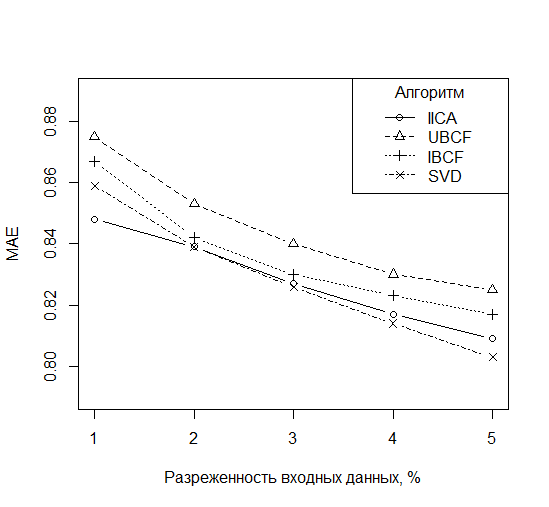
\includegraphics[width=1\linewidth]{MAE-density} \\ а)}
	\end{minipage}
	\hfill
	\begin{minipage}[h]{0.49\linewidth}
	\center{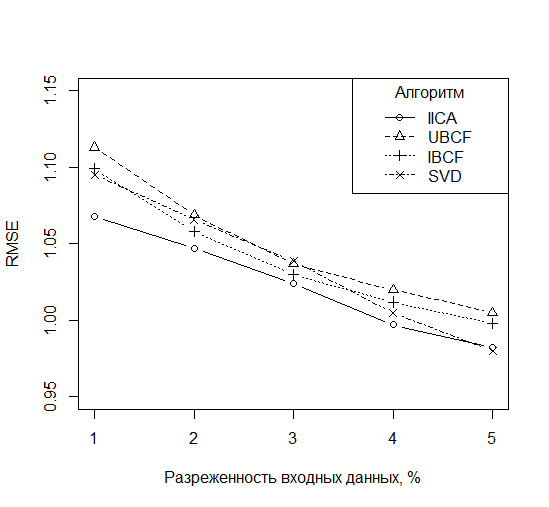
\includegraphics[width=1\linewidth]{rmse-sparsity} \\ б)}
	\end{minipage}
	\caption{Зависимость качества работы системы от разреженности входных данных.}
	\label{fig:accuracy}
	\end{figure}
	\par
	Во всех предыдущих тестов пороговое качество кластеризации было положено равным 2. Это обусловлено предварительным тестированием работы системы. На Рис. \ref{fig:accuraccur} показана зависимость RMSE и MAE описанного алгоритма в зависимости от порогового значения точности кластеризации. 
	
	\begin{figure}[h]
	\begin{minipage}[h]{0.49\linewidth}
	\center{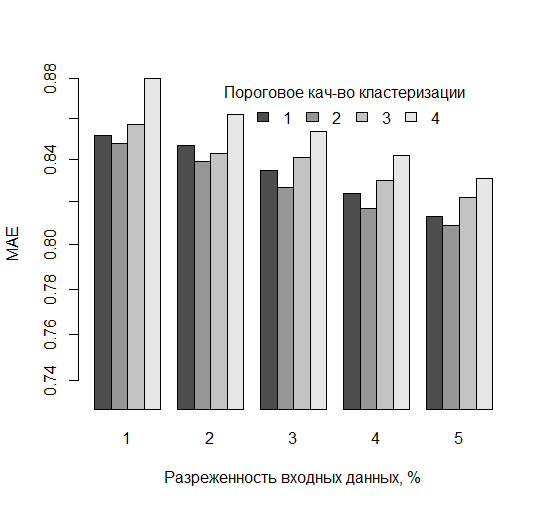
\includegraphics[width=1\linewidth]{Rplotmae} \\ а)}
	\end{minipage}
	\hfill
	\begin{minipage}[h]{0.49\linewidth}
	\center{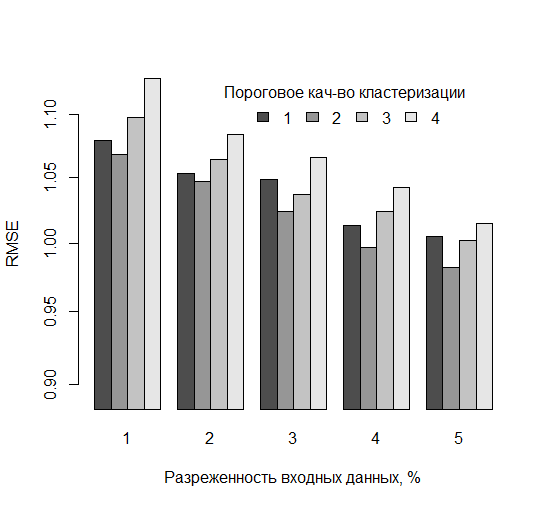
\includegraphics[width=1\linewidth]{Rplotrmse} \\ б)}
	\end{minipage}
	\caption{Зависимость качества работы системы от порогового значения точности кластеризации.}
	\label{fig:accuraccur}
	\end{figure}
	Значение коэффициента нечеткости $r$ на основе предварительного тестирования было положено равным 1,5 . На Рис. \ref{fig:fuzz} показана зависимость RMSE и MAE описанного алгоритма в зависимости от значения коэффициента нечеткости. Во время тестирования системы и определения оптимального значения этого параметра было положено $\hat{K}=2$. 
	\begin{figure}[h!]
	\begin{minipage}[h]{0.49\linewidth}
	\center{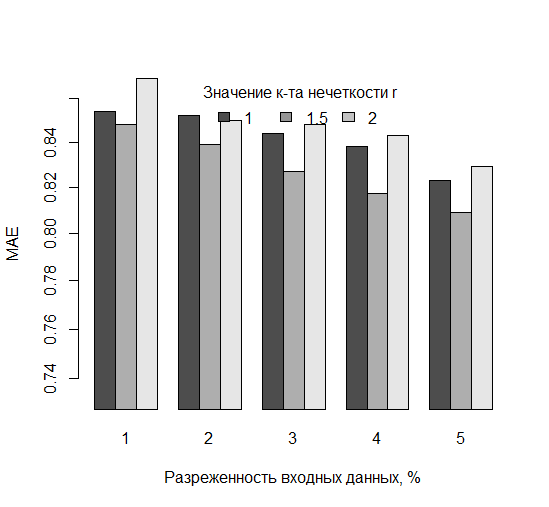
\includegraphics[width=1\linewidth]{Rplot_mae_fuzz} \\ а)}
	\end{minipage}
	\hfill
	\begin{minipage}[h]{0.49\linewidth}
	\center{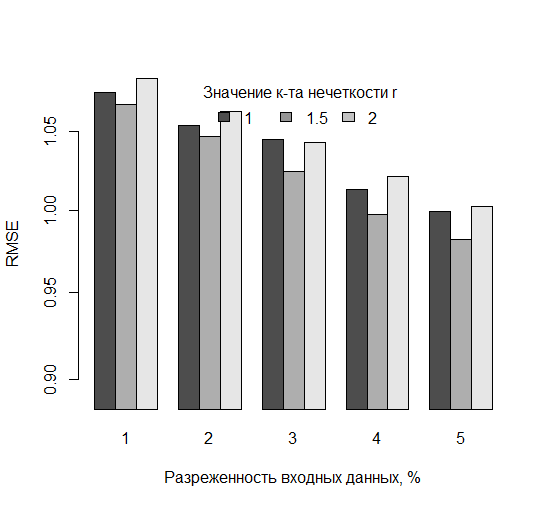
\includegraphics[width=1\linewidth]{Rplot_rmse_fuzzyness} \\ б)}
	\end{minipage}
	\caption{Зависимость качества работы системы от значения коэффициента нечеткости $r$.}
	\label{fig:fuzz}
	\end{figure}

\par
	

\section{Заключение}
В работе был представлен рекомендательный алгоритм, основной задачей которого является повышение качества рекомендаций при работе со входными данными высокой разреженности. Для этого предлагается использовать итерационный алгоритм, на каждом шаге которого происходит оценка части неизвестных рейтингов, после чего кластеризуются пользователи системы. Тестовые результаты показали, что на данных высокой разреженности предложенный алгоритм действительно превосходит наиболее популярные рекомендательные методы по такому параметру, как качество оценки неизвестных рейтингов.  
К недостаткам полученного алгоритма можно отнести высокую вычислительную сложность, обусловленную многократным использованием кластеризации.
\par
Полученный алгоритм был реализован на языке программирования R\footnote{См. раздел <<Приложение>>}.

\newpage
\cleardoublepage

\addcontentsline{toc}{section}{Список литературы}
\begin{thebibliography}{99}
\bibitem{bees} Ju C., Xu C. A New Collaborative Recommendation Approach Based on Users Clustering Using Artificial Bee Colony Algorithm //The Scientific World Journal. – 2013. – Т. 2013.

\bibitem{hash} Кольчугина Е. А., Макарь В. А. Метод коллаборативной фильтрации для масштабируемых рекомендательных систем //Современные научные исследования и инновации. – 2012. – №. 6. – С. 4.

\bibitem{smoothing} Adomavicius G., Zhang J. Iterative Smoothing Technique for Improving Stability of Recommender Systems //Workshop on Recommendation Utility Evaluation: Beyond RMSE (RUE 2011). – 2012. – С. 3.

\bibitem{itercf} Zhang Z., Cuff P., Kulkarni S. Iterative collaborative filtering for recommender systems with sparse data //Machine Learning for Signal Processing (MLSP), 2012 IEEE International Workshop on. – IEEE, 2012. – С. 1-6.

%\bibitem{hybrid} кластеризация для гибридных РС
\bibitem{fanny} Kaufman L., Rousseeuw P. J. Finding groups in data: an introduction to cluster analysis. – John Wiley \& Sons, 2009. – Т. 344.

\bibitem{coldstart} Schein A. I. et al. Methods and metrics for cold-start recommendations //Proceedings of the 25th annual international ACM SIGIR conference on Research and development in information retrieval. – ACM, 2002. – С. 253-260.

\bibitem{cfbasedsvd} Sarwar B. et al. Application of dimensionality reduction in recommender system-a case study. – Minnesota Univ Minneapolis Dept of Computer Science, 2000. – №. TR-00-043.

\bibitem{empiricalanalysis} Breese J. S., Heckerman D., Kadie C. Empirical analysis of predictive algorithms for collaborative filtering //Proceedings of the Fourteenth conference on Uncertainty in artificial intelligence. – Morgan Kaufmann Publishers Inc., 1998. – С. 43-52.

%\bibitem{fuzzycmeans} Pattern Recognition with Fuzzy Objective Function Algoritms

\bibitem{socnetclust} Pham M. C. et al. A Clustering Approach for Collaborative Filtering Recommendation Using Social Network Analysis //J. UCS. – 2011. – Т. 17. – №. 4. – С. 583-604.

\bibitem{cfdef} Adomavicius G., Tuzhilin A. Toward the next generation of recommender systems: A survey of the state-of-the-art and possible extensions //Knowledge and Data Engineering, IEEE Transactions on. – 2005. – Т. 17. – №. 6. – С. 734-749.

\bibitem{neighbourhoodselection} Zhang J., Pu P. A recursive prediction algorithm for collaborative filtering recommender systems //Proceedings of the 2007 ACM conference on Recommender systems. – ACM, 2007. – С. 57-64.

\bibitem{clustersearch} Altingovde I. S., Subakan Ö. N., Ulusoy Ö. Cluster searching strategies for collaborative recommendation systems //Information Processing \& Management. – 2013. – Т. 49. – №. 3. – С. 688-697.

\bibitem{clusteritemcf} O’Connor M., Herlocker J. Clustering items for collaborative filtering //Proceedings of the ACM SIGIR workshop on recommender systems. – UC Berkeley, 1999. – Т. 128.

\bibitem{grouplens} Resnick P. et al. GroupLens: an open architecture for collaborative filtering of netnews //Proceedings of the 1994 ACM conference on Computer supported cooperative work. – ACM, 1994. – С. 175-186.

\end{thebibliography}

\newpage
\section{Приложение}
\subsection{Исходный код программы}

\begin{lstlisting}[language=R]

# extra packages
install.packages('cluster')
library('cluster')

# userA, userB - vectors of user ratings
pearson_similarity <- function(userA, userB) {
  
  #average ratings given by users A and B
  r_a <- mean(userA, na.rm=TRUE)
  r_b <- mean(userB, na.rm=TRUE)
  
  co_rated <- (!is.na(userA) & !is.na(userB)) 
  co_rated_indexes <- c(1:length(userA))[co_rated]
  
  a <- 0
  b <- 0
  c <- 0
  for (i in co_rated_indexes) {
    a <- a + (userA[i] - r_a) * (userB[i] - r_b)
    b <- b + (userA[i] - r_a) ^ 2
    c <- c + (userB[i] - r_b) ^ 2
  }
  if (b == 0) {
    return (0.5 * sign(a))
  }
  if (c == 0) {
    return(0.5 * sign(a))
  }
  return (a / (sqrt(b) * sqrt(c))) 
}

# userA, userB - vectors of user ratings
cosine_similarity <- function(userA, userB) {
  
  co_rated <- (!is.na(userA) & !is.na(userB)) 
  
  scalar_product <- sum(userA[co_rated] * userB[co_rated])
  norm_a <- sqrt(sum(userA[co_rated]^2))
  norm_b <- sqrt(sum(userB[co_rated]^2))
  return(scalar_product / (norm_a * norm_b))
}

# returns numbers of clusters whose membership 
# degrees together are greater than degree 
# array - vector of  degrees of cluster membership
# degree - level of clusterization accuracy
best_clust <- function(array, degree=0.8) { 
  degrees_and_class <- array
  degrees_and_class <- rbind(degrees_and_class,
   c(1:length(array)))
  ord <- order(degrees_and_class[1,], decreasing = TRUE)
  degrees_and_class <- degrees_and_class[,ord]
  sum <- 0
  res <- 1
  repeat {
    sum <- sum + degrees_and_class[1,res]
    if (sum >= degree) {
      break
    } else {
      res <- res + 1
    }
  }
  return(degrees_and_class[2,1:res])
}

# creating similarity matricix between users
create_similarity_matrix <- function(rating_matrix, method="pearson", ...) {
  res <- matrix(0, nrow(rating_matrix), nrow(rating_matrix))
  if (method == "pearson") {

    for (i in 1:nrow(rating_matrix)) {
      for (j in 1:i) {
        res[i, j] <- pearson_similarity(rating_matrix[i,],
         rating_matrix[j,])      
      }
    }
    
    
  } else if (method == "cosine") {
    for (i in 1:nrow(rating_matrix)) {
      for (j in 1:nrow(rating_matrix)) {
        res[i, j] <- cosine_similarity(rating_matrix[i,],
         rating_matrix[j,])      
      }
    }
  } 
  for (i in 1:nrow(res)) {
    for (j in i: nrow(res))
      res[i,j] <- res[j,i]
  }
  res[is.na(res)] <- 0
  return(res)
}

# creates new matrix leaving only rows who belong to the clusters
# data - rating matrix
# clustering - vector of positive integers,  clusters of users
# clusters - clusters we want to leave
cut_data_matrix <- function(data, clustering, clusters) { 
  result <- data[1,] # the line we want to predict is the first line
  
  for (i in 2:nrow(data)) {
    if (clustering[i] %in% clusters) { 
      result <- rbind(result, data[i,])
    }
  }
  return (result)
}


# matrix - rating matrix
# row_number - positive integer
# similarity - double vector
# mean_user_ratings - double vector
# users_who_rated - boolean matrix
# ratings_to_estimate - boolean vector
# check - additional stuff for debugging
# co_rated_bound - integer
# return_na - bool
estimate_user <- function(matrix, row_number, similarity,
 mean_user_ratings, users_who_rated, ratings_to_estimate,
  co_rated_bound, return_na, check = "0") { 
  print("estimation started")
  print(Sys.time())
  if (nrow(matrix) == 1) { # matrix = vector 
    result <- matrix
    mean_user_rating <- mean(matrix[1,], na.rm = TRUE)
    for (i in 1: ncol(matrix)) {
      if (is.na(matrix[1,i])) {
        result[1,i] <- mean_user_rating
      }
    }
    return(result)
  } 
  
  estimated_matrix <- matrix
  mean_rating <- mean_user_ratings[row_number]
  estimated_user <- c()

  for (l in 1: ncol(estimated_matrix)) {  

    if (ratings_to_estimate[l]) { # estimate missing rating r_{1l} -
     only for current user
      
      users_who_rated_item_l <- users_who_rated[,l] 
      if (sum(users_who_rated_item_l) <= co_rated_bound) {
        if (return_na) { 
          estimated_user <- c(estimated_user, NA)
        } else {
          estimated_user <- c(estimated_user, mean_rating )
        }
      } else {

        mean_user_ratings_who_rated_item_l <-
         mean_user_ratings[users_who_rated_item_l] 

        item_l_ratings <-
         estimated_matrix[users_who_rated_item_l, l]  
 
        diff_ratings <- item_l_ratings -
         mean_user_ratings_who_rated_item_l
 
        sim_users_who_rated_item_l <-
         similarity[users_who_rated_item_l]
        sum_dist <- sum(abs(sim_users_who_rated_item_l)) 
        
        if (sum_dist == 0) {
          estimated_rating <- 0
        } else {
          estimated_rating <- sum(sim_users_who_rated_item_l  *
           diff_ratings) / sum_dist
        }
        
        print(Sys.time())
        estimated_user <- c(estimated_user, mean_rating +
         estimated_rating)
      }
    } else {
      estimated_user <- c(estimated_user,
       estimated_matrix[row_number, l])
    } 
  } 
  return(estimated_user)
}

# main function for ratings predictions 
# data - training rating matrix
# test - testing set
# clust_num - clustering accurace threshold
# total_clust_num - number of clusters on start
# clust_weight - level of clusteriztion accuracy
predict <- function(data, test = NULL, clust_num = 2,
 total_clust_num = 10, clust_weight = 0.7, max_iterations = 20,
  cluster_shift = -1, min_clust_size =  10,method = "pearson") {
  print(Sys.time())
  print("started")
  result_matrix <- c()
  
  if (!is.null(test)) {
    print("testing set found")
    print("estimating only users in test set")
    users_to_estimate = nrow(test)
  } else {
    print("testing set not found")
    print("estimateing all users")
    users_to_estimate = nrow(data)
  }
  
  data <- rbind(test, data)
  
  default_similarity_matrix <- (create_similarity_matrix(data,
   method = method)) 
  default_distance_matrix <- 1 / (default_similarity_matrix +
   1.001)
  default_fanny <- fanny(as.dist(default_distance_matrix),
   total_clust_num, maxit = 20000, memb.exp = 1.5)
  default_clustering <- default_fanny['clustering'][[1]]
  default_membership <- default_fanny['membership'][[1]]
  default_clusters <- lapply(split(default_membership,
   seq(nrow(default_membership))), best_clust)
  
  print(Sys.time())
  print("preprocessing finished")
  
  for (i in 1:users_to_estimate) {
    number_of_clusters <- length(default_clusters[[i]]) 
    
    ## moving estimated user to the first row to the sake of
    # convenience
    estimated_matrix <- rbind(data[i,], data[-i,])
    clustering <- c(default_clustering[i],default_clustering[-i])
    membership <- rbind(default_membership[i,],
     default_membership[-i,])
    clusters <- default_clusters[[i]]
    similarity <- c(default_similarity_matrix[i,i],
     default_similarity_matrix[i,-i])
    
    tmp <- default_similarity_matrix[-i,-i]
    similarity_matrix <- rbind(similarity[-1], tmp)
    similarity_matrix <- cbind(similarity, similarity_matrix)
    iteration <- 0
    
    max_clust_num <- clust_num
    
    ratings_to_estimate <- is.na(estimated_matrix[1,])
    
    repeat { # estimate ratings 

      copy <- estimated_matrix
      estimated_matrix <- cut_data_matrix(estimated_matrix,
       clustering, clusters)
      good_users <- clustering %in% clusters # we don't compute
      # dist matrix again but get it from existing one by leaving #only those users who are in good clusters 
      similarity <- similarity[good_users]

      similarity_matrix <- similarity_matrix[good_users,
       good_users] 

      if (is.null(dim(estimated_matrix))) {
        estimated_matrix <- t(as.matrix(estimated_matrix))
      }
      new_estimated_matrix <- estimated_matrix

      mean_user_ratings <- apply(estimated_matrix, 1, mean,
       na.rm = TRUE)
      mean_user_ratings[is.na(mean_user_ratings)] <- 0 
      
      users_who_rated <- !apply(estimated_matrix, 1:2, is.na)
      
      new_estimated_matrix[1,] <-
       estimate_user(estimated_matrix, 1, similarity_matrix[1,],
        mean_user_ratings, users_who_rated, ratings_to_estimate,
         0, FALSE, similarity_matrix) 
      if (number_of_clusters <= max_clust_num || iteration ==
       max_iterations || nrow(estimated_matrix) <=
        min_clust_size) { 

        break
      } else { #and recompute clustering and get new
       number_of_user_clusters
        max_clust_num <- number_of_clusters + cluster_shift
        for (k in 2: nrow(estimated_matrix)) {

          new_estimated_matrix[k,] <-
           estimate_user(estimated_matrix, k, similarity_matrix[k,],
            mean_user_ratings, users_who_rated,
             is.na(estimated_matrix[k,]), 2, TRUE)
        }
        
        similarity_matrix <-
         create_similarity_matrix(new_estimated_matrix, method = method)
        distance_matrix <- 1 / (similarity_matrix + 1.001)
        fanny <- fanny(as.dist(distance_matrix), total_clust_num,
         maxit = 20000, memb.exp = 1.5)
        clustering <- fanny['clustering'][[1]]
        membership <- fanny['membership'][[1]]
        clusters_all <- lapply(split(membership,
         seq(nrow(membership))), best_clust)
        clusters <- clusters_all[[1]]
        number_of_clusters <- length(clusters[[1]])
        iteration <- iteration + 1
        estimated_matrix <- new_estimated_matrix
        similarity <- similarity_matrix[1,]
        
      } 
    }
    result_matrix <- rbind(result_matrix,
     new_estimated_matrix[1,])
  }
  return(result_matrix) 
}
\end{lstlisting}


\end{document}

